\documentclass[a4paper, french, 10pt]{article}
\usepackage{babel}
\usepackage[left = 3 cm, right = 3 cm, top = 2 cm, bottom = 2 cm]{geometry}
% \usepackage{python}
\usepackage{makeidx}
\usepackage{fontspec}
\setmainfont{Linux Libertine}
\setsansfont{Linux Biolinum}
\setmonofont{Consolas}
\usepackage{color}
%\rmfamily % To load Latin Modern Roman and enable the following NFSS declarations.
% Declare that Latin Modern Roman (lmr) should take
% its bold (b) and bold extended (bx) weight, and small capital (sc) shape,
% from the corresponding Computer Modern Roman (cmr) font, for the T1 font encoding.
%\DeclareFontShape{T1}{lmr}{b}{sc}{<->ssub*cmr/bx/sc}{}
%\DeclareFontShape{T1}{lmr}{bx}{sc}{<->ssub*cmr/bx/sc}{}
\usepackage[colorlinks=true]{hyperref}
\hypersetup{urlcolor=blue,linkcolor=black,citecolor=blue,colorlinks=true}
\usepackage{sectsty}
\allsectionsfont{\bfseries\sffamily}
\usepackage{caption}
\usepackage{graphicx}
\setlength\parindent{0pt}
\newcommand{\code}[1]{{\small\texttt{#1}}}
\makeindex
\usepackage{minted}
\definecolor{mygreen}{rgb}{0,0.6,0}
\definecolor{myblue}{rgb}{0,0,1}
\usepackage{titlesec}
\usepackage{titletoc}
\setcounter{tocdepth}{2}
\reversemarginpar
\usepackage{enumitem}
\title{Mémo Python}

\titlecontents
	{section}
	[0em]
	{\bfseries\addvspace{0.5em}}
	{\bfseries{\thecontentslabel.\ }}
	{}
	{\hfill\bfseries\contentspage}
	[\addvspace{0pt}]

\titlecontents
	{subsection}
	[1em]
	{\addvspace{0.25em}}
	{\thecontentslabel.\ }
	{}
	{\hfill\contentspage}
	[\addvspace{0pt}]

\begin{document}

\begin{center}
        {\Huge{\sc\bfseries{Mémo Python}}}\\[20pt]
        
\includegraphics[scale=0.1]{python.png}
        \vspace{20pt}
\end{center}
\tableofcontents
\hypersetup{linkcolor=blue}

\paragraph{Remarque}
 Ne sont pas reprises les opérations \og basiques \fg{} (boucles, manipulation des listes). On s'intéresse directement à la programmation orientée objet. Ensuite sont détaillés quelques fonctionnalités apportées par des modules.

\part{Programmation orientée objet en Python}
\section{Constantes et types natifs}
 Quelques constantes sont définies par Python comme \code{True}\index{True} et \code{False}\index{False}. De la même manière, quelques classes sont définies par défaut, appeléss types natifs, comme:
\begin{enumerate}
		\item Types booléens
		\begin{enumerate}
			\item Booléen (\href{https://docs.python.org/fr/3/library/functions.html?highlight=bool#bool}{\code{bool}})
			\item Opérations booléennes (\href{https://docs.python.org/fr/3/library/stdtypes.html#boolean-operations-and-or-not}{\code{and, or, not}})
		\end{enumerate}
        \item Types numériques
        \begin{enumerate}
              \item Entier (\href{https://docs.python.org/fr/3/library/stdtypes.html#typesnumeric}{\code{int}})
              \item Flottant (\href{https://docs.python.org/fr/3/library/stdtypes.html#typesnumeric}{\code{float}})
              \item Complexe (\href{https://docs.python.org/fr/3/library/stdtypes.html#typesnumeric}{\code{complex}})
      \end{enumerate}
     \item Types séquentiels
	\begin{enumerate}
       \item Liste (\href{https://docs.python.org/fr/3/library/stdtypes.html#sequence-types-list-tuple-range}{\code{list}})
		\item Tuple (\href{https://docs.python.org/fr/3/library/stdtypes.html#sequence-types-list-tuple-range}{\code{tuple}})
		\item Range (\href{https://docs.python.org/fr/3/library/stdtypes.html#sequence-types-list-tuple-range}{\code{range}})
	\end{enumerate}
        \item Chaîne de caractères (\href{https://docs.python.org/fr/3/library/string.html?highlight=str#module-string}{\code{str}})
		\item Séquences binaires (\href{https://docs.python.org/fr/3/library/stdtypes.html#binary-sequence-types-bytes-bytearray-memoryview}{\code{bytes, bytearray, memoryview}})
		\item Ensemble (\href{https://docs.python.org/fr/3/library/stdtypes.html#set-types-set-frozenset}{\code{set}} (muable), \href{https://docs.python.org/fr/3/library/stdtypes.html#set-types-set-frozenset}{\code{frozenset}} (non muable))
		\item Dictionnaire (\href{https://docs.python.org/fr/3/library/stdtypes.html#mapping-types-dict}{\code{dict}})
\end{enumerate}
La liste n'est pas exhaustive, des compléments sur les types natifs sont disponibles dans la documentation.
\paragraph{Documentation} Documentation Python 3: \href{https://docs.python.org/fr/3/library/constants.html}{constantes natives}, \href{https://docs.python.org/fr/3/library/stdtypes.html}{types natifs}
\section{Variables}\index{variable}


\section{Classes}\index{classe}
 Les classes permettent des créer des objets\index{objet} appelés instances\index{instance}) qui partagent des caractéristiques de leur classe. Une classe correspond donc à un type, ou plutô à un gabarit d'objet.

\paragraph{Documentation} \href{https://openclassrooms.com/courses/apprenez-a-programmer-en-python/premiere-approche-des-classes}{Introduction OpenClassrooms}, \href{https://docs.python.org/fr/3/tutorial/classes.html}{Documentation Python 3}, \href{https://fr.wikibooks.org/wiki/Programmation_Python/Classes#Définition_d'une_classe_élé mentaire}{Wikilivres}
\subsection{Structure d'une classe}
Les objets d'une classe partagent des caractéristiques communes à la classe: des attributs\index{attribut} et des méthodes (des fonctions qui agissent sur leur attributs). Les objets sont créés g\^ace à une méthode spéciale appelée constructeur.

\subsubsection{Création}
Pour créer une classe, la syntaxe est la suivante:
\begin{minted}[fontsize = \footnotesize, frame = single]{python}
class MaClasse:
    <contenu>
\end{minted}

Si la classe hérite d'une classe mère, alors il faut l'ajouter en argument:
\begin{minted}[fontsize = \footnotesize, frame = single]{python}
class MaClasse(ClasseMere):
    <contenu>
\end{minted}

\subsubsection{Initialiseur}\index{initialiseur}\index{\_\_init\_\_}

L'initialiseur est une méthode spéciale appelée \Verb[fontsize = \small]|__init__|, il prend en argument \code{self}\index{self} (toutes les méthodes de la classe prennent en argument \code{self} qui est en fait l'instance en question) et tous les paramètres nécessaires à l'initialisation de l'instance. Il ne s'agit pas du constructeur (même si on l'appelle parfois ainsi par abus de langage) : il ne crée  pas à proprement parler l'instance, mais agit sur celle-ci lorsqu'elle vient d'être créée. Le \og véritable \fg{} constructeur est la méthode \code{\_\_new\_\_}, il n'est en général pas nécessaire de l'implémenter, sauf par exemple lorsque l'on crée des \hyperref[sec:metaclasses]{métaclasses} ou si l'on veut créer des classes qui héritent des types natifs. L'initialiseur est appelé automatiquement lors que l'on crée l'objet (après le constructeur).
\begin{minted}[fontsize = \footnotesize, frame = single]{python}
class MaClasse:
    CONSTANTE = ...
    def __init__(self, att1, att2):
        """Initialiseur"""
        self.attribut_1 = att1
        self.attribut_2 = att2
        self.attribut_3 = CONSTANTE
\end{minted}
Ici, les deux premiers attributs sont personnalisables lors de la création des objets alors que le dernier est commun à tous. \code{CONSTANTE} est une variable de classe\index{variable de classe}. Pour créer un objet on écrit simplement:
\begin{minted}[fontsize = \footnotesize, frame = single]{python}
objet = MaClasse(att1, att2)
\end{minted}

\subsubsection{Méthodes}\index{méthode}
Les méthodes se définissent comme des fonctions, elles agissent en général sur les instances de la classe. Elles doivent prendre \code{self} en argument :
\begin{minted}[fontsize = \footnotesize, frame = single]{python}
class MaClasse:
    def __init__(self):
         <contenu>

    def methode(self, arg1, arg2):
         <contenu>
\end{minted}

Ensuite on les appelle de la manière suivante:
\begin{minted}[fontsize = \footnotesize, frame = single]{python}
objet.methode(arg1, arg2)
\end{minted}


\subsection{Héritage}\index{héritage}

L'héritage est un moyen de créer des classes dérivées (classes filles) d'une classe source (classe mère). Une classe fille hérite de toutes les méthodes et variables de sa classe mère. Pour créer une classe fille, on utilise la syntaxe suivante.

\begin{minted}[frame = single, fontsize = \footnotesize]{python}
class Mere:
    <contenu>

class Fille(Mere):
    <contenu>
\end{minted}

Il est possible d'écraser une méthode héritée en la redéfinissant dans la classe fille. Si on veut accéder à une méthode héritée alors qu'on l'a redéfinie dans la classe fille, on utilise la fonction \code{super()} qui permet d'appeler la méthode de la classe mère de la classe présente (sans l'argument self).

\paragraph{Exemple}
\begin{minted}[frame = single, fontsize = \footnotesize]{python}
class Meuble:
    def __init__(self, couleur, materiau):
        self.couleur = couleur
        self.materiau = materiau

class Bibliotheque(Meuble):
    def __init__(self, couleur, materiau, n):
        super().__init__(couleur, materiau)
        self.nb_livres = n
\end{minted}
On peut utiliser deux fonctions pour vérifier l'héritage: \code{isinstance} renvoie \code{True} si l'objet est une instance de la classe ou de ses classes filles ; \code{issubclass} permet de voir si une classe est fille d'une autre.

\begin{Verbatim}[frame = single, fontsize = \footnotesize]
>>> bibli = Bibliotheque('blanc', 'vert', 150)
>>> bibli.__dict__
{'couleur': 'blanc', 'materiau': 'vert', 'nb_livres': 150}
>>> isinstance(bibli, Meuble)
True
>>> isinstance(bibli, Bibliotheque)
True
>>> issubclass(Bibliotheque, Meuble)
True
>>> issubclass(Meuble, Bibliotheque)
False
>>> isinstance(bibli, int)
False
>>> isinstance(bibli, object)
True
\end{Verbatim}

\paragraph{Documentation} \href{https://openclassrooms.com/courses/apprenez-a-programmer-en-python/l-heritage-9}{OpenClassrooms}, \href{https://docs.python.org/fr/3/tutorial/classes.html?highlight=héritage#inheritance}{Documentation Python 3}, \href{https://www.programiz.com/python-programming/inheritance}{Programiz}
\subsection{Méthodes spéciales}\index{méthode spéciale}
 Les méthodes spéciales sont déjà définies par défaut dans Python mais on peut les personnaliser. Elles sont reconnaissables par leur typographies: leur nom commence et se termine par deux soulignés.

\paragraph{Documentation} \href{https://docs.python.org/3/reference/datamodel.html#specialnames}{Documentation Python 3}, \href{https://openclassrooms.com/courses/apprenez-a-programmer-en-python/les-methodes-speciales-1}{OpenClassrooms}


\subsubsection{Construction, initialisation et destruction}
Le constructeur est la méthode \code{\_\_new\_\_}. C'est une \hyperref[sec:classmethod]{méthode de classe} qui prend en argument \code{cls} et les autres arguments qui seront en paramètres de l'initialiseur; il doit retourner un objet (l'instance à créer). \code{\_\_init\_\_} a déjà été décrit précédemment (contrairement au constructeur, cette méthode ne retourne rien). En pratique, on n'implémente pas la méthode \code{\_\_new\_\_} sauf dans certains cas.

\paragraph{Exemple} On veut définir une classe \og singleton \fg{} qui ne peut créer qu'une instance.

\begin{minted}[frame = single, fontsize = \footnotesize]{python}
class Singleton:
    """Classe qui ne peut instancier qu'une fois."""

    instance = None

    def __new__(cls, *args, **kwargs):
        if instance is None:
            cls.instance = super().__new__(cls, *args, **kwargs)
            return cls.instance
        else:
            raise TypeError("Cette classe singleton possède déjà une instance")

    def __init__(self, *args, **kwargs):
        pass
\end{minted}

Pour détruire un objet, on définit la méthode \code{\_\_del\_\_}\index{\_\_del\_\_}. On l'appelle comme ceci:
\begin{minted}[fontsize = \footnotesize, frame = single]{python}
del objet
\end{minted}

\subsubsection{Représentation et chaine de caractère d'un objet}
Il existe deux méthodes spéciales nommées \code{\_\_repr\_\_}\index{\_\_repr\_\_} et \code{\_\_str\_\_}\index{\_\_str\_\_} qui sont appelées lorsque l'on exécute \code{repr(objet)} ou \code{return objet}, et quand on exécute \code{str(objet)} ou bien \code{print(objet)}. La fonction \code{\_\_repr\_\_} est donc utilisée lorsque l'on veut avoir accès à la représentation d'un objet, tandis que \code{\_\_str\_\_} permet de présenter l'objet de manière plus élégante en chaine de caractères. Ces deux fonctions prennent en argument \code{self}. Lorsque la méthode \code{\_\_str\_\_} n'est pas définie, Python appelle la fonction de représentation à la place.

\paragraph{Exemple} L'exemple suivant
\begin{minted}[fontsize = \footnotesize, frame = single]{python}
class MaClasse:
    def __init__(self):
         self.attribut = 'Exemple'

    def __repr__(self):
        return "MaClasse({})".format(self.attribut)

    def __str__(self):
        return "Instance de MaClasse ayant comme attribut {}"
              .format(self.attribut)
\end{minted}
permet de faire:
\begin{Verbatim}[fontsize = \footnotesize, frame = single]
>>> obj = MaClasse()
>>> obj
MaClasse(Exemple)
>>> print(obj)
Instance de MaClasse ayant comme attribut Exemple.
\end{Verbatim}

\subsubsection{Accesseur et mutateur}\index{accesseur}\index{mutateur}\index{destructeur}
Lorsque Python essaie d'accéder à un attribut, il appelle en premier la méthode spéciale \code{\_\_getattribute\_\_}\index{\_\_getattribute\_\_}, puis il appelle les \hyperref[sec:proprietes]{descripteurs} s'il sont définis. Lorsque l'on veut modifier un attribut, c'est la méthode spéciale \code{\_\_setattr\_\_}\index{\_\_setattr\_\_} puis les descripteurs qui sont appelés. Si on essaie d'accéder à un attribut non défini, Python appelle en guise de dernière chance la méthode \code{\_\_getattr\_\_}\index{\_\_getattr\_\_}. On peut personnaliser cette fonction de manière à ce qu'elle envoie une erreur, ou bien à ce qu'elle redirige vers un autre attribut ou effectue un calcul.

\paragraph{Exemple}
\begin{minted}[frame = single, fontsize = \footnotesize]{python}
class MaClasse:
    def __init__(self)
        self.a = int()

    def __getattribute__(self, attribut):
        print("J'accède à l'attribut {}...".format(attribut))
        return object.__getattribute__(self, attribut)

    def __getattr__(self, attribut):
        print("L'attribut {} est inaccessible !".format(attribut))

    def __setattr__(self, attribut, valeur):
        object.__setattr__(self, attribut, valeur)
        print("L'attribut a été changé !")
        # Il est nécessaire d'appeler la méthode par défaut, car appeler self.__setattr__
        # donnerait une récursivité infinie. En fait, on ne sait à ce stade pas comment
        # Python change concrètement la valeur de l'attribut.
\end{minted}

On note que l'on utilise les méthodes spéciales de la classe \code{object} (méthodes par défaut) car appeler \code{self.\_\_getattribute\_\_} ou \code{self.\_\_setattr\_\_} donnent une récursivité sans fin ! Cela permet de faire:
\begin{Verbatim}[fontsize = \footnotesize, frame = single]
>>> objet = MaClasse()
L'attribut a été changé !
>>> objet.b
L'attribut b est inaccessible !
>>> objet.a
J'accède à l'attribut a...
0
>>> objet.attribut = 1
L'attribut a été changé !
>>> objet.a
J'accède à l'attribut a...
1
\end{Verbatim}
Il existe aussi \code{\_\_delattr\_\_}\index{\_\_delattr\_\_} qui prend en arguments \code{self} et le nom de l'attribut. Cette méthode est appelée lorsque l'on effectue \code{del objet.attribut}. Lors de l'écriture de la méthode, il faut utiliser \code{object.\_\_delattr\_\_} de la même manière que l'on utilise \code{object.\_\_setattr\_\_} pour \code{\_\_setattr\_\_} ou \code{object.\_\_getattribute\_\_} pour \code{\_\_getattribute\_\_}.\bigskip

\subsubsection{Méthodes de conteneur}\index{méthode de conteneur}\index{conteneur}
Il existe trois méthodes (accesseur, mutateur, destructeur) qui permettent d'agir sur l'objet avec l'opérateur \code{[]} (utilisé pour les listes par exemple). Dans ce cas, l'objet peut être un conteneur qui contient d'autres objets. Le fonctionnement de ses méthodes est similaires aux précédentes. Sont définies en outre \code{\_\_contains\_\_}\index{\_\_contains\_\_} qui permet de déterminer si un élément est présent ou non dans le conteneur (retourne un booléen) et \code{\_\_len\_\_}\index{\_\_len\_\_} qui retourne la longueur du conteneur. Tableau récapitulatif:
\begin{center}
        \begin{tabular}{|p{2.5cm}|p{3.5 cm}|p{5cm}|}
        \hline
        \multicolumn{1}{|c}{\bf Méthode} & \multicolumn{1}{|c}{\bf Arguments} & \multicolumn{1}{|c|}{\bf Appel} \\
        \hline
        \code{\_\_getitem\_\_} & \code{self, index} & \code{conteneur[index]}\\
        \hline
        \code{\_\_setitem\_\_} & \code{self, index, valeur} & \code{conteneur[index] = valeur}\\
        \hline
        \code{\_\_delitem\_\_} & \code{self, index} & \code{del conteneur[index]}\\
        \hline
        \code{\_\_contains\_\_} & \code{self, element} & \code{element in conteneur}\\
        \hline
        \code{\_\_len\_\_} & \code{self} & \code{len(conteneur)}\\
        \hline
\end{tabular}
\end{center}

\subsubsection{Surcharges d'opérateur}\index{surcharge d'opérateur}
Les surcharges d'opérateur permettent de faire des opérations arithmétiques avec des objets, c'est-à-dire d'indiquer à Python ce qu'il faut faire lorsque l'on exécute \code{objet1 + objet2}. Ces méthodes prennent en arguments \code{self} (l'objet 1) et l'objet 2.
\begin{center}
\begin{tabular}{|p{2.5cm}|c|}
        \hline
        \multicolumn{1}{|c|} {\bf Méthode} & {\bf Appel}\\
        \hline
        \code{\_\_add\_\_}\index{\_\_add\_\_} & \code{objet1 + objet2}\\
        \hline
        \code{\_\_sub\_\_}\index{\_\_sub\_\_} & \code{objet1 - objet2}\\
        \hline
        \code{\_\_mul\_\_}\index{\_\_mul\_\_} & \code{objet1 * objet2}\\
        \hline
        \code{\_\_truediv\_\_}\index{\_\_truediv\_\_} & \code{objet1 / objet2}\\
        \hline
        \code{\_\_floordiv\_\_}\index{\_\_floordiv\_\_} & \code{objet1 // objet2}\\
        \hline
        \code{\_\_mod\_\_}\index{\_\_mod\_\_} & \code{objet1 \% objet2}\\
        \hline
\end{tabular}
\end{center}
Les deux objets ne sont pas nécessairement du même type ! Cependant, cette opération n'est pas symétrique : le code \code{objet + 5} par exemple exécute \code{objet.\_\_add\_\_(5)}, alors que \code{5 + objet} exécute \code{int.\_\_add\_\_(5)}. Pour que l'opération soit symétrique, il faut aussi définir ces fonctions avec le préfixe \code{r} (par exemple \code{\_\_radd\_\_}).
\subsection{Méthodes statiques et méthodes de classes}
\subsubsection{Méthode statique}\index{méthode statique}
Les méthodes que l'on a vues jusqu'à maintenant agissent sur les instances des classes : elles prennent toujours en premier argument le mot clé \code{self} qui renvoie à l'instance elle même. Lorsque l'on appelle une telle méthode sur une instance comme ceci:
\mintinline[fontsize=\small]{python}
{instance.methode(<arguments>)},
Python exécute en fait \code{Classe.methode(instance, <arguments>)}.\bigskip

En fait, ces deux objets sont différents. \code{Classe.methode} est une simple fonction, alors que \code{instance.methode} est une méthode évaluée sur l'instance (en anglais \og bound method \fg{}\index{bound method}), c'est-à-dire que l'instance est mise en premier argument. On considère cet exemple:

\paragraph{Exemple}
\begin{minted}[frame=single, fontsize=\footnotesize]{python}
class Maths:

    def addition(x, y):
        return x + y

    def multiplication(x, y):
        return x * y

    def division(x, y):
        return x / y
\end{minted}
On choisit ici de grouper trois fonctions car elles sont logiquement liées. Elles n'influent pas les instances donc elles ne prennent pas \code{self} en argument. Si l'on appelle ces méthodes sur une instance, une exception sera levée car Python entrera automatiquement l'argument \code{self} (donc en tout trois arguments) alors que les méthodes n'en prennent que deux. Pour remédier à cela, on les décore avec \code{@staticmethod}. On peut maintenant les appeler indifféremment sur la classe ou sur des instances.

\subsubsection{Méthode de classe}\index{méthode de classe}\label{sec:classmethod}
Lorsque l'on veut manipuler des variables de classe et non des attributs d'instances, on crée des méthodes de classe. Celles-ci prennent la classe en premier argument, par convention on le note \code{cls}; elles ne prennent logiquement pas \code{self} comme argument. Cette méthode est donc évaluée sur la classe. Sans autre modification, on ne peut peut appeler cette méthode que sur les instances car Python attend l'argument \code{cls}. Pour pouvoir appeler cette méthode sur la classe (logique car c'est une méthode de classe), on la décore avec \code{@classmethod}.

\subsubsection{Cas de l'héritage}
En résumé:
\begin{enumerate}
        \item Les méthodes statiques sont des fonctions reliées à des classes, mais qui n'agissent pas sur celles-ci.
        \item Les méthodes de classe sont des fonctions qui prennent la classe en paramètre.
\end{enumerate}

Une classe qui hérite d'une classe mère hérite de toutes ses méthodes. Les méthodes statiques restent donc inchangées, tandis que les méthodes de classe s'adaptent à la nouvelle classe, car elles la prennent en premier argument.

\paragraph{Exemple} Un exemple d'utilisation de méthodes statiques et de classe sont la création de constructeurs alternatifs. On s'aperçoit de la différence des deux notions.
\begin{minted}[frame=single, fontsize=\footnotesize]{python}
class Personne:
    def __init__(self, nom, age):
        self.nom = nom
        self.age = age

    @staticmethod
    def par_date_de_naissance(nom, date):
        return Personne(nom, 2018-date)

    @classmethod
    def par_date_de_naissance2(cls, nom, date):
        return cls(nom, 2018-date)

class Homme(Personne):
    sexe = 'homme'
\end{minted}
\begin{Verbatim}[frame=single, fontsize=\footnotesize]
>>> homme1 = Homme.par_date_de_naissance('Jean', 1997)
>>> homme2 = Homme.par_date_de_naissance2('Jean', 1997)
>>> type(homme1)
<class '__main__.Personne'>
>>> type(homme2)
<class '__main__.Homme'>
\end{Verbatim}

Pour avoir \code{homme1} de type \code{Homme}, il faut redéfinir la méthode statique dans la classe fille.

\paragraph{Documentation} \href{https://www.programiz.com/python-programming/methods/built-in/staticmethod}{Méthode statique sur Programiz}, \href{https://www.programiz.com/python-programming/methods/built-in/classmethod}{Méthode de classe sur Programiz}, \href{https://stackoverflow.com/questions/136097/what-is-the-difference-between-staticmethod-and-classmethod-in-python/1669524#1669524}{StackOverflow}


\subsection{Propriétés}\label{sec:proprietes}\index{propriété}\index{accesseur}\index{mutateur}\index{destructeur}
 Les propriétés représentent en Python le principe d'encapsulation. Elles sont utiles si on souhaite contrôler l'accès à un attribut ou si on veut que le changement d'une valeur d'un attribut engendre des modifications sur d'autres attributs. Les propriétés sont un cas particulier des descripteurs.

\subsubsection{Définition d'une propriété}

On crée les propriétés en utilisant des décorateurs. Elles contiennent un accesseur, un mutateur, un destructeur et une aide (docstring de l'accesseur).\bigskip

Les propriétés sont aussi un moyen de simuler des attributs privés: pour simuler un attribut privé, on précède son nom d'un souligné. Ainsi, on appelle cet attribut sans le souligné dans le code g\^ace aux propriétés. Par convention, on n'agit pas sur les attributs qui commencent par un souligné en Python.

\paragraph{Exemple}
\begin{minted}[fontsize = \footnotesize, frame = single]{python}
class MaClasse:
    def __init__(self):
        self._attribut = 'Je suis un attribut'

    @property
    def attribut(self):
        """Propriété 'attribut'."""
        print("Accès à l'attribut")
        return self._attribut

    @attribut.setter
    def attribut(self, valeur):
        print("Modification de l'attribut")
        self._attribut = valeur

    @attribut.deleter
    def attribut(self):
        print('Adieu :(')
        del self._attribut
\end{minted}

On utilise la propriété de la manière suivante:
\begin{Verbatim}[frame = single, fontsize = \footnotesize]
>>> instance = MaClasse()
>>> instance.attribut
Accès à l'attribut
'Je suis un attribut'
>>> instance.attribut = 'Ah bon ?'
Modification de l'attribut
>>> del instance.attribut
Adieu :(
>>> help(MaClasse.attribut)
Help on property:

    Propriété 'attribut'.

\end{Verbatim}

\paragraph{Documentation}\href{https://docs.python.org/fr/3/library/functions.html?highlight=property#property}{Documentation Python 3}, \href{https://stackoverflow.com/questions/15750522/class-properties-and-setattr/15751159#15751159}{Priorités entre propriété et méthodes spéciales}
\subsubsection{Généralisation: les descripteurs}
On dit qu'un objet est un descripteur s'il possède au moins une méthode \code{\_\_get\_\_} (accesseur), \code{\_\_set\_\_} (mutateur), ou \code{\_\_delete\_\_} (destruteur).

\paragraph{Exemple} Exemple d'implémentation
\begin{minted}[frame = single, fontsize = \footnotesize]{python}
class Attribut:
    def __get__(self, inst, insttype):
        print("Accès à l'attribut")
        return inst._attribut

    def __set__(self, inst, valeur):
        print("Modification de l'attribut")
        inst._attribut = valeur

class MaClasse:
    def __init__(self):
        self._attribut = 'Je suis un attribut'

    attribut = Attribut()
\end{minted}

\paragraph{Documentation} \href{https://docs.python.org/3/howto/descriptor.html}{Documentation Python 3}

\section{Itérateurs}\index{itérateur}
\section{Générateurs}\index{générateur}
\section{Décorateurs}\index{décorateur}
Les décorateurs sont des fonctions ou des classes qui permettent de modifier le comportement d'une autre fonction (ou classe). Les décorateurs sont utiles lorsque l'on souhaite qu'un certain nombre de fonctions effectuent des tâches communes comme par exemple donner leur temps d'exécution. On appelle un décorateur de la manière suivante.

\begin{minted}[fontsize = \footnotesize, frame = single]{python}
@decorateur
def fonction():
    pass
\end{minted}

Le code précédent a le même comportement que le code suivant.

\begin{minted}[fontsize = \footnotesize, frame = single]{python}
def fonction():
    pass

fonction = decorateur(fonction)
\end{minted}

Ainsi, \code{fonction} devient l'objet retournée par \code{decorateur(fonction)}. Le décorateur doit donc retourner un objet que l'on peut appeler en écrivant \code{objet()} (avec d'éventuels arguments), on appelle ce type d'objet un \og callable\fg{}\index{callable}. Le décorateur est bien sûr lui même un callable. Si on le définit comme une classe, on doit définir la méthode \code{\_\_call\_\_} qui permet de rendre ses instances callable.

\paragraph{Documentation} \href{https://stackoverflow.com/questions/739654/how-to-make-a-chain-of-function-decorators/1594484#1594484}{Stack Overflow}

\subsection{En tant que classe}
Une façon d'implémenter un décorateur est d'utiliser les classes. La fonction décorée deviendra alors une instance de la classe de ce décorateur. Il faut obligatoirement définir la méthode \code{\_\_call\_\_} pour pouvoir rendre cette instance callable.

\paragraph{Exemple} On considère ici un décorateur qui compte le nombre d'appels de la fonction décorée.
\begin{minted}[frame = single, fontsize = \footnotesize]{python}
class Compteur:
    def __init__(self, f):
        self.call = 0
        self.f = f

    def __call__(self, *args, **kwargs):
        self.call += 1
        print("La fonction {} a été appelée {} fois.".format(self.f.__name__, self.call))
        return self.f(*args, **kwargs)
\end{minted}
\subsection{En tant que fonction}
Comme un décorateur est un objet callable qui n'a d'autre utilité que d'être appelé, il est aussi logique de le définir en tant que fonction.

\paragraph{Exemple} Même décorateur que précédemment mais en l'implémentant en tant que fonction.
\begin{minted}[fontsize = \footnotesize, frame = single]{python}
def compteur(f):
    def wrapper(*args, **kwargs):
        wrapper.call += 1
        print("La fonction {} a été appelée {} fois.".format(f.__name__, wrapper.call))
        return f(*args, **kwargs)
    wrapper.call = 0
    return wrapper
\end{minted}
\paragraph{Remarques} On voit dans cet exemple que l'on peut définir des fonctions dans les définitions de fonctions. La mention \code{*args} fait référence à tous les arguments non nommés que l'on a entrés (c'est un tuple, par exemple \code{(arg1, arg2)}). La mention \code{**kwargs} fait référence aux arguments nommés (c'est un dictionnaire). Ainsi on est sûr de récupérer tous les arguments.\bigskip

Dans cet exemple, on assigne à \code{wrapper} un attribut de fonction (on peut le faire, puisqu'une fonction est un objet -- de la classe \code{function}). On le définit après avoir défini cette fonction.

\subsection{Décorateurs à paramètres}
On peut faire en sorte que le décorateur prenne un ou plusieurs paramètres. Dans ce cas, il faut définir le décorateur à l'intérieur d'une clôture qui prend en argument ces différents paramètres.

\paragraph{Exemple} On veut retourner une erreur quand la fonction retourne une valeur trop élevée.
\begin{minted}[frame = single, fontsize = \footnotesize]{python}
def depasse_max(max):
    def deco(f):
        def wrapper(*args, **kwargs):
            n = f(*args, **kwargs)
            if n > max:
                print("Maximum {} dépassé.".format(max))
                return
            return n
        return wrapper
    return deco
\end{minted}

Ces deux syntaxes sont équivalentes:

\begin{minted}[frame = single, fontsize = \footnotesize]{python}
@depasse_max(10)
def demande_nombre():
    n = int(input("Entrer un nombre : "))
    return n

def demande_nombre():
    n = int(input("Entrer un nombre : "))
    return n

demande_nombre = depasse_max(10)(demande_nombre)
\end{minted}

Cela permet de faire

\begin{Verbatim}[frame = single, fontsize = \footnotesize]
>>> demande_nombre()
Entrer un nombre : 11
Maximum 10 dépassé.
\end{Verbatim}

\section{Métaclasses}\index{métaclasse}\label{sec:metaclasses}
Les métaclasses sont les classes qui instancient d'autres classes. Par défaut, une seule métaclasse est définie : la métaclasse \code{type}. On s'en rend compte en demandant le type des classes que l'on crée.

\begin{minted}[frame = single, fontsize = \footnotesize]{python}
class MaClasse:
    pass

print(type(MaClasse)) # <class 'type'>
\end{minted}

\setcounter{section}{0}

\newpage
\part{Modules}
\section{Librairie standard}

\subsection{re}\index{re}\index{expression régulière}
Le module \code{re} permet d'utiliser les expressions régulières en Python.
\paragraph{Documentation} \href{https://docs.python.org/fr/3/library/re.html}{Documentation Python 3}

\subsubsection{Ecrire une expression régulière}
Les expressions régulières sont un excellent moyen de retrouver des motifs complexes dans une chaine de caractères. On écrit les motifs à rechercher grâce à plusieurs caractères spéciaux:
\begin{description}
    \item [Spécification du caractère]~
    \begin{itemize}
        \item \og\code{.}\fg{} désigne n'importe quel caractère.
        \item \og\code{[]}\fg{} permet de dire quels caractères on veut trouver (\code{[a-e]} : \code{a}, \code{b}, \code{c}, \code{d} ou \code{e}; \code{[a-eA-E]} idem avec les majuscule comprises; \code{[+-*]}: soit \code{*} soit \code{+} soit \code{-}).
        \item \og\Verb[fontsize=\small]|\w|\fg{} équivaut à \Verb[fontsize=\small]|[a-zA-Z0-9_]|.
        \item \og\Verb[fontsize=\small]|\W|\fg{} désigne tout caractère non alpha-numérique.
        \item \og\Verb[fontsize=\small]|\d|\fg{} équivaut à \code{[0-9]}.
        \item \og\Verb[fontsize=\small]|\D|\fg{} désigne tout caractère non numérique.
        \item \og\Verb[fontsize=\small]|\s|\fg{} désigne un espace.
    \end{itemize}
    \item [Place du motif dans la chaine]~
    \begin{itemize}
        \item \og\Verb[fontsize=\small]!^!\fg{} (se place au début) signifie que le début de la chaine doit correspondre au motif.
        \item \og\code{\$}\fg{} (se place à la fin) signifie que la fin de la chaine doit correspondre au motif.
    \end{itemize}
    \item [Nombre d'apparition(s) consécutive(s)]~
    \begin{itemize}
        \item \og\code{\{n\}}\fg{} indique que le caractère précédent doit apparaitre \code{n} fois.
        \item \og\code{\{n,m\}}\fg{} indique que le caractère précédent doit apparaitre entre \code{n} et \code{m} fois.
        \item \og\code{*}\fg{} indique que le caractère précédent n'apparait pas ou apparait sans maximum d'occurences (\code{ab*} correspond à \code{a}, \code{ab}, ou bien \code{abbbbbb}, etc.).
        \item \og\code{+}\fg{} indique que le caractère précédent apparait au moins une fois (\code{ab+} correspond à \code{ab}, \code{abb}, ou bien \code{abbbbbb}, etc.).
        \item \og\code{?}\fg{} indique que le caractère précédent apparait au plus une fois (équivalent à \code{\{0,1\}}).
    \end{itemize}
\end{description}

Les quatre derniers qualificateurs sont dits gourmands : ils valident autant de caractères que possible. Par exemple pour \code{"aaaaa"}, \code{a\{3,5\}} validera la chaine en entier. Pour une version non gourmande, on suit le qualificateur d'un \code{?} : \code{*?}, \code{+?}, \code{??} et \code{\{n,m\}?}. Un qualificateur non gourmand valide le moins de caractères possibles.\bigskip

Pour contrôler le nombre d'apparitions d'un groupe de caractères, on met ceux-ci entre parenthèses (\code{(abc)+}: \code{abc}, \code{abcabc}, etc.). Cela crée un groupe de caractères, on peut le nommer en suivant la parenthèses ouvrante de \code{?P<nom>}. Cela est utile par exemple quand on veut remplacer des caractères. On peut séparer des expression régulières par un \code{|} afin d'indiquer que plusieurs possibilités sont possibles.\bigskip

\subsubsection{Méthodes}
On compile une expression régulière en utilisant la fonction \code{compile}\marginpar{re.compile}. Cette fonction retourne un objet expression régulière (regex) sur lequel on peut évaluer diverses méthodes. Si l'on cherche une phrase, la syntaxe sera:

\begin{minted}[frame = single, fontsize = \footnotesize]{python}
import re

regex = re.compile(r"[A-Z]\w*\s?(\w+\s?)*.")
\end{minted}

\paragraph{Remarque} On utilise le préfixe \code{r} devant la chaine de caractère pour éviter d'avoir à écrire \Verb[fontsize = \small]|\\| au lieu d'un unique \Verb[fontsize = \small]|\|.\bigskip

On peut rechercher toutes les occurences du motif grâce à la méthode \code{re.finditer(motif, chaine)}\marginpar{regex.finditer}. Cela retourne un objet iterable. On accède aux objets en appelant \code{next(iterable)}, qui retourne un objet expression rationnelle. Celui-ci contient plusieurs chaines de caractères (une pour chaque groupe du motif), on y accède en appelant les différents groupes : \code{objet.group(numéro ou nom)}.\bigskip

\paragraph{Exemple} On veut extraire les phrases d'une chaîne de caractères.
\begin{description}
\item[Script]~

\begin{minted}[frame = single, fontsize = \footnotesize]{python}
chaine = r"Je suis une phrase. Moi aussi"
regex = re.compile(r"[A-Z]\w*\s?(?:\w+\s?)*.")
resultats = regex.finditer(chaine)
while True:
    try:
        print(next(resultats).group(0))
    except:
        break
\end{minted}
\item[Sortie]~

\begin{Verbatim}[frame = single, fontsize = \footnotesize]
Je suis une phrase.
Moi aussi.
\end{Verbatim}
\end{description}

On peut remplacer les motifs par d'autres motifs en utilisant la méthode \code{re.sub}\marginpar{regex.sub}. Elle prend en paramètres:
\begin{enumerate}
    \item le motif (chaîne de caractères ou objet expression rationnelle.)
    \item le remplacement (peut être une fonction)
    \item la chaine à traiter
    \item \code{count=}le nombre d'occurences à remplacer
\end{enumerate}
et renvoie la chaine de caractères modifiée. Lorsque l'on veut appeler un groupe de caractères nommé avec \code{(?P<nom>)}, on y fait référence dans la chaine de remplacement par \Verb[fontsize = \small]|\g<nom>|.

\paragraph{Exemple}
\begin{minted}[frame = single, fontsize = \footnotesize]{python}
pass
\end{minted}



\subsection{datetime}\index{datetime}

Le module \code{datetime}\marginpar{\code{datetime}} permet de créer des objets représentant des dates et de faire des opérations. La classe \code{datetime.date} représente une date par son année, son mois et son jour: \code{jour = datetime.date(2017, 1, 1)} correspond à la date 1\ier{} janvier 2017.
La classe \code{datetime.timedelta} permet de faire des opérations sur les dates. Ses objets sont représentés par un nombre de jours (on peut construire un \code{timedelta} avec des semaines/mois/années, le constructeur convertit en jours).
Le module \code{datetime} peut ausi être utilisé pour utiliser des durées plus réduites, i.e.\ secondes, minutes, heures, etc.

\paragraph{Exemple}
\begin{Verbatim}[fontsize = \footnotesize, frame = single]
>>> import datetime
>>> j1 = datetime.date(2017, 1, 1)
>>> j2 = j1 + datetime.timedelta(30)
>>> j2
datetime.date(2017, 1, 31)
\end{Verbatim}


\paragraph*{Documentation} \href{https://docs.python.org/fr/3/library/datetime.html}{Documentation Python 3}

\subsection{turtle}\index{turtle}

Contient des classes pour dessiner des formes simples en faisant avancer des tortues. Elles peuvent avancer, reculer, tourner d'un certain angle.
La classe \code{Turtle} permet de créer des objets tortues qui peuvent :
\begin{enumerate}
        \item Avancer: \code{Turtle.forward(<nb de pixels>)}
        \item Reculer: \code{Turtle.backward(<nb de pixels>)}
        \item Tourner à droite ou à gauche (ex: \code{Turtle.right(<degrés>)})
        \item Changer de couleur (\code{Turtle.color(<couleur>)}) ou de forme (\code{Turtle.shape(<forme>)}).
\end{enumerate}

\paragraph{Exemple}
\begin{minted}[fontsize = \footnotesize, frame = single]{python}
import turtle

Terrain = turtle.Screen()
Terrain.bgcolor("black")

Tortue = turtle.Turtle()
Tortue.speed(3)
Tortue.shape("turtle")
Tortue.color("white")

for i in range(50):
    for e in range(4):
        Tortue.forward(100)
        Tortue.right(90)
    Tortue.right(360/50)

Terrain.exitonclick()
\end{minted}

\begin{figure}[h]
\begin{center}
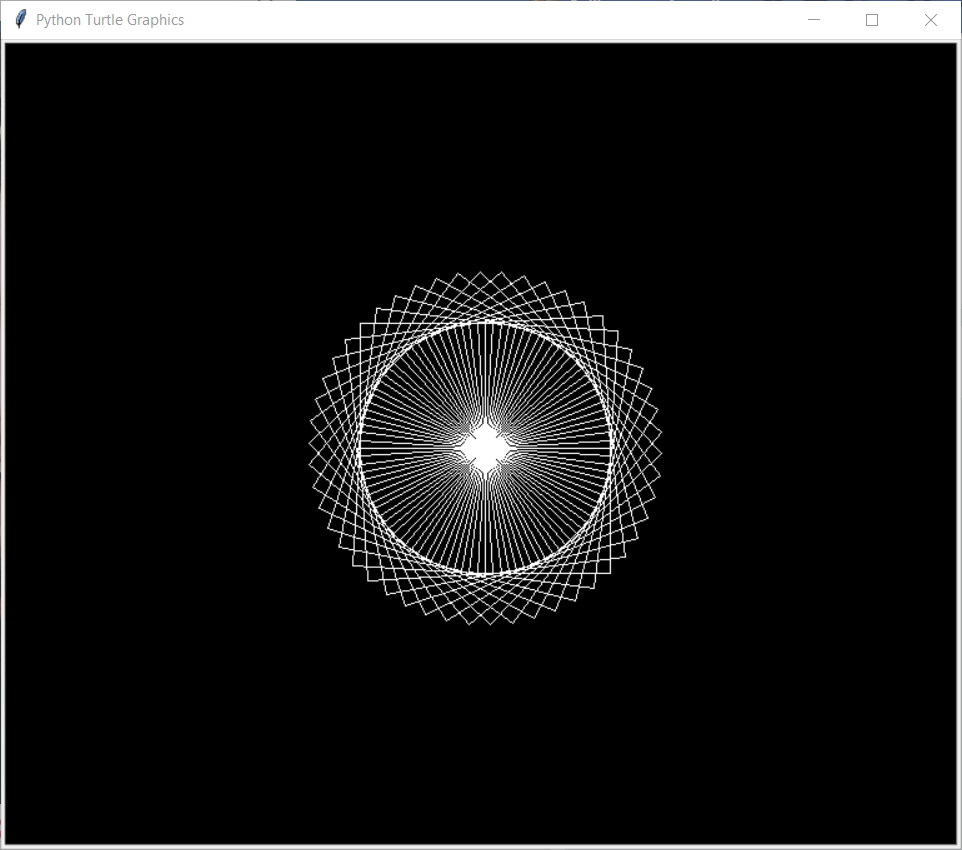
\includegraphics[scale=0.5]{turtle.png}
\caption*{Résultat}
\end{center}
\end{figure}

\paragraph{Documentation} \href{https://docs.python.org/fr/3.6/library/turtle.html#methods-specific-to-screen-not-inherited-from-turtlescreen}{Documentation Python 3}, \href{https://fr.wikibooks.org/wiki/Programmation_Python/Turtle}{Wikilivres}

\subsection{ctypes}\index{ctypes}
 Ce module sert à appeler des fonctions écrites en langage C dans des librairies DLL par exemple.
\subsubsection{Boites de dialogue}\index{boîte de dialogue}
 Le module ctypes peut servir à faire apparaitre des boites de dialogue. On peut modifier le comportement du script Python en fonction du bouton appuyé car la fonction faisant apparaitre ces boites renvoie un entier qui dépend du bouton appuyé. Diverses options sont disponibles :
\begin{minted}[fontsize = \footnotesize, frame = single]{python}
# Button styles:
# 0 : OK
# 1 : OK | Annuler
# 2 : Abandonner | Recommencer | Ignorer
# 3 : Oui | Non | Annuler
# 4 : Oui | Non
# 5 : Recommencer | Annuler
# 6 : Annuler | Recommencer | Continuer

# To also change icon, add these values to previous number
# 16 Icone erreur
# 32 Icone question
# 48 Icone attention
# 64 Icone information
\end{minted}

\paragraph{Exemple}
\begin{minted}[fontsize = \footnotesize, frame = single]{python}
ctypes.windll.user32.MessageBoxW(0, "That's an error", "Warning!", 16)
\end{minted}
\begin{figure}[h]
\begin{center}
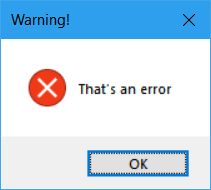
\includegraphics[scale=0.5]{errorwindow.png}
\caption*{Résultat}
\end{center}
\end{figure}

\subsection{keyboard}\index{keyboard}
\subsection{os}\index{os}
\subsection{sys}\index{sys}


\section{Modules à télécharger}
\subsection{twilio}\index{twilio}
\subsection{win10toast}\index{win10toast}
\subsection{splinter}\index{splinter}
\subsection{pylint}\index{pylint}

\subsection{autopy}\index{autopy}


%\addcontentsline{toc}{section}{Index}
\printindex
\end{document}
